\documentclass[border=4pt]{standalone}
% Preámbulo común de las figuras. Cada figura es un documento standalone
% que se compila a SVG con scripts/build_figures.sh
\usepackage[utf8]{inputenc}
\usepackage{amsmath}
\usepackage{tikz}
\usepackage[american, siunitx]{circuitikz}
\usetikzlibrary{arrows.meta,calc,decorations.pathmorphing,patterns}
\tikzset{
  >={Stealth[length=2.2mm]},
  eje/.style={->, thin},
  hilo/.style={thick},
}
% Paleta común: tonos medios legibles sobre fondo claro
\definecolor{azul}{RGB}{31,94,168}
\definecolor{rojo}{RGB}{192,57,43}
\definecolor{verde}{RGB}{39,128,73}
\definecolor{naranja}{RGB}{211,120,30}
\definecolor{morado}{RGB}{125,60,152}

\begin{document}
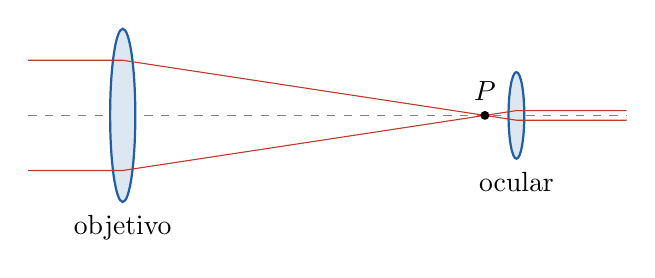
\begin{tikzpicture}[scale=1.0]
  \draw[dashed, gray] (-1.2,0) -- (6.4,0);
  \filldraw[draw=azul, fill=azul!15, thick] (0,0) ellipse (0.16 and 1.1);
  \filldraw[draw=azul, fill=azul!15, thick] (5.0,0) ellipse (0.1 and 0.55);
  \draw[rojo] (-1.2,0.7) -- (0,0.7) -- (4.6,0) -- (5.0,-0.061) -- (6.4,-0.061);
  \draw[rojo] (-1.2,-0.7) -- (0,-0.7) -- (4.6,0) -- (5.0,0.061) -- (6.4,0.061);
  \fill (4.6,0) circle (1.6pt) node[above=2pt]{$P$};
  \node[below] at (0,-1.15) {objetivo};
  \node[below] at (5.0,-0.6) {ocular};
\end{tikzpicture}
\end{document}
